%Ezequiel França dos Santos
%Artigo - BCC - SENAC
\documentclass[12pt]{article}
\usepackage{sbc-template}
\usepackage{graphicx,url}
\usepackage[brazil]{babel}   
\usepackage[utf8]{inputenc}  
\usepackage{graphicx,url}
\usepackage[portuges, brazil]{babel}   
\usepackage[utf8]{inputenc}
\usepackage{listings}
\usepackage{xcolor}
\usepackage{natbib}
\definecolor{dkgreen}{rgb}{0,0.6,0}
\definecolor{dred}{rgb}{0.545,0,0}
\definecolor{dblue}{rgb}{0,0,0.545}
\definecolor{lgrey}{rgb}{0.9,0.9,0.9}
\definecolor{gray}{rgb}{0.4,0.4,0.4}
\definecolor{darkblue}{rgb}{0.0,0.0,0.6}
\usepackage{listings}
\lstdefinelanguage{cpp}{
      backgroundcolor=\color{white},  
      basicstyle=\footnotesize \ttfamily \color{black} \bfseries,   
      breakatwhitespace=false,       
      breaklines=true,               
      captionpos=b,                   
      commentstyle=\color{dkgreen},   
      deletekeywords={...},          
      escapeinside={\%*}{*)},                  
      frame=single,                  
      language=C,                
      keywordstyle=\color{purple},  
      morekeywords={BRIEFDescriptorConfig,string,TiXmlNode,DetectorDescriptorConfigContainer,istringstream,cerr,exit}, 
      identifierstyle=\color{black},
      stringstyle=\color{blue},      
      numbers=none,                 
      numbersep=5pt,                  
      numberstyle=\tiny\color{black}, 
      rulecolor=\color{black},        
      showspaces=false,               
      showstringspaces=false,        
      showtabs=false,                
      stepnumber=1,                   
      tabsize=5,                     
      title=\lstname,                 
    }

%comando para mudar a enumeração do listing para código
\renewcommand{\lstlistingname}{Código}    
    
    
\sloppy

\title{LogiKid - Proposta de um jogo educativo para o ensino de portas lógicas}
\author{Ezequiel França dos Santos\inst{1}, Gabriel Fontenelle Senna\inst{1}, Tales Carlos de Pádua\inst{1} }
\address 
{Centro Universitário Senac - Campus Santo Amaro
  (SENAC-SP)\\
  Av. Engenheiro Eusébio Stevaux, 823 -- Santo Amaro, São Paulo -- CEP 04696-000 -- SP -- Brasil
%\nextinstitute
%  Departamento de Tecnologia da Informação\\
%  Bacharelado em Ciência da Computação
  \email{{ezefranca.br,colecionador.gabriel,talescpadua},{(@gmail.com})}
}

\begin{document} 
\maketitle
\begin{abstract}
This paper presents results for the development of an educational computer game called LogiKid,  where the objective is the teaching and learning of logic gates and Boolean logic. Accordingly, the present paper focuses on the description of how it was built and show the way of visual presentation of the concepts of logic gates, as proposed educational objectives. The development involved issues such as learning time, ludica approach and also relevant issues for a game, as their yours challenges and technical aspects of coding.
\end{abstract}
     
\begin{resumo} 
O presente artigo apresenta os resultados relativos ao desenvolvimento de um jogo eletrônico educativo, chamado
LogiKid, voltado para o ensino e aprendizagem de portas logicas e logica booleana. Neste sentido, o presente tra-
balho enfoca a descrição de como foi incorporada ao jogo a apresentação de maneira visual dos conceitos de portas logicas, conforme objetivos educacionais propostos. O
desenvolvimento envolveu questões como tempo de aprendizado, abordagem lúdica e também questões pertinentes
a um jogo, como seus desafios e aspectos técnicos na programação.
\end{resumo}


\section{Introdução}
Os jogos educativos digitais possibilitam a criação de ambientes de
aprendizagem atraentes e gratificantes, constituindo-se num recurso poderoso de
estímulo para o desenvolvimento do jogador, permitindo o desenvolvimento de
inúmeras habilidades. A temática do jogo é o ensino de portas lógicas, na era da tecnologia a importância dessas portas lógicas está no fato de representarem os elementos básicos de construção da maioria dos circuitos digitais, das lógicas computacionais e em diversas outras aplicações.

%-------------------------------------------------------------------------------------------------------------------------------------------------%
\section*{Desenvolvimento de um jogo educativo} \label{sec:gamedev}

\subsection{Jogos Educativos}
Os jogos educativos digitais possibilitam a criação de ambientes de
aprendizagem atraentes e gratificantes, constituindo-se num recurso poderoso de estímulo para o jogador, permitindo o desenvolvimento de inúmeras habilidades. 

\subsection{Elementos pedagógicos e lúdicos dos jogos}
O significado atual do jogo na educação, sinaliza a existência  de divergências em torno do jogo educativo, que estaria relacionado concomitamente a duas funções:
A primeira seria a função lúdica do jogo, expressa na ideia de que sua vivência propicia a diversão, o prazer, quando escolhido voluntariamente pelo individuo. A segunda seria a função educativa que representa a maneira de ensinar.[1]
O  jogo é mais do que um fenômeno fisiológico ou um reflexo psicológico, o jogo "é uma função significante, isto é, encerra um determinado sentido".[2] 

%-------------------------------------------------------------------------------------------------------------------------------------------------%
\section{Metodologia}
O jogo foi desenvolvido utilizando a Linguagem de Programação C, padrão C99, e a biblioteca Allegro 5. 

\subsection{Linguagem C padrão C99}

Um dos recursos da C99 utilizado neste trabalho foi o tipo booleano. Incluindo a stdbool.h, podemos declarar variáveis do tipo bool e usar os estados verdadeiro e falso, assim:
\begin{lstlisting}[language=cpp,caption={{Demonstração do tipo bool na linguagem C\\\\}}]
#include <stdbool.h>

void main()
{
   bool var;

   if (var)
      var = false;
}
\end{lstlisting}
É fato que isso já era feito usando-se 1 e 0 e na verdade os estados true e false não passam de outros nomes (#define) para estes números, respectivamente. No entanto, a legibilidade do código melhora com o tipo bool.


\subsection{Biblioteca Allegro5}
A Allegro é uma das bibliotecas mais populares entre as pessoas que se iniciam na programação de jogos virtuais para
computadores. Tal popularidade se justifica pelo fato dela proporcionar acesso fácil às
rotinas comumente necessárias no desenvolvimento de jogos virtuais, tais como entrada de mouse, teclado e joystick, geração de gráficos, efeitos sonoros e gerenciamento
de tempo (timers). Além disso, a biblioteca se destaca por ser livre, sem custos de
licença de uso para o desenvolvedor.[3] 

\subsection{Aspectos técnicos do jogo}\label{sec:figs}

Na codificação do jogo, foi utilizada uma metodologia 
estruturada, com uso de funções, criando estruturas para criação de telas e a game engine. 
A \textbf{Figura 1} mostra o diagrama da arquitetura adotada.

\begin{figure}[ht]
\centering
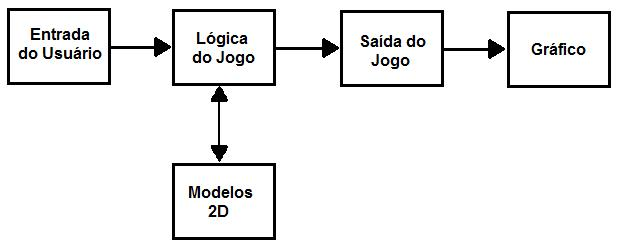
\includegraphics[width=.5\textwidth]{diagrama.jpg}
\caption{Arquitetura do jogo}
\label{fig:exampleFig3}
\end{figure}
A construção das fases contemplou um design didático, semelhante a programas de simulação de circuitos, como Logisim[5] por exemplo.
O fato de trabalharmos com circuitos lógicos possibilitou o uso dos próprios operadores da linguagem C
para criação da lógica do jogo, pois ela possui todos operadores lógicos necessários para este fim. O trecho de código abaixo exemplifica este uso.
\begin{lstlisting}[language=cpp,caption={{Exemplo de código para atribuição com Allegro 5, utilizando operadores lógicos da linguagem C}}]
void drawLogicLevel(bool gateOne, bool gateTwo, Level *level){
	if(!gateOne && !gateTwo) 
	level->circ1 = al_load_bitmap("./data/00XX.png");
	if(!gateOne && gateTwo) 
	level->circ1 = al_load_bitmap("./data/01XX.png");
	if(gateOne && !gateTwo) 
	level->circ1= al_load_bitmap("./data/10XX.png");
	if(gateOne && gateTwo)  
	level->circ1 = al_load_bitmap("./data/11XX.png");
}
\end{lstlisting}
\section{Considerações Finais}

Para este trabalho foi muito importante o estudo dos conceitos de portas lógicas, necessários para
planejar como seria o desenvolvimento do jogo Logikid. Foram abordados desde conceitos
básicos até aos conceitos de circuitos avançados. A partir desse
estudo foi possível criar o jogo Logikid, mediante os requisitos um jogo educativo.
O resultado final, foi um jogo simples e interativo  e de grande impacto visual.
Com os estudos realizados foi possível notar a vantagem do uso de softwares
educativos no processo de ensino, pois o computador facilita o uso de atividades de ensino-aprendizagem
pelo professor. Porém um jogo educativo deve ser projetado e desenvolvido com qualidade, pois sem um boa base pedagógica e lúdica pode acabar servindo apenas de distração para o
aluno e um jogo sem uma interface de qualidade pode fazer com que o aluno não
se motive à utilizá-lo.
\section*{}
\bibliographystyle{sbc}
\begin{thebibliography}{1}

\bibitem{KISHIMOTO}
Tizuko Kishimoto.
  {\em O jogo e a educaçao Infantil}, 
  Cengage Learning, Sao Paulo, 2008.

\bibitem{Maria Carmen Silveira Barbosa}
Maria Carmen Silveira Barbosa.
\newblock Jogo, brinquedo, brincadeira e a educação.
\newblock {\em Educ. Soc. [online]}, Scielo, pg:398--404, 1997.

\bibitem{Allegro Manual}
[Online].
\newblock Allegro 5.0 reference manual.
\newblock {\em $<$https://www.allegro.cc/manual/5/$>$ }
\newblock {\em Acesso em Outubro de 2013}.

\bibitem{GIT}
GIT.
\newblock Manual de Referência.
\newblock {\em $<$http://git-scm.com/docs$>$}
\newblock {\em Acesso em Outubro de 2013}.

\bibitem{Logisim}
BURCH, Carl
\newblock Documentação do Software LogiSim.
\newblock {\em $<$http://ozark.hendrix.edu/burch/logisim/pt/docs.html$>$ }
\newblock {\em Acesso em Novembro de 2013}.

\bibitem{Kris Shaffer}
Kris Shaffer.
\newblock Push, Pull, Fork: GitHub for Academics.
\newblock {\em $<$http://hybridpedagogy.com/Journal/GitHubforAcademics$>$}
\newblock {\em Acesso em Novembro de 2013}.

\bibitem{Hu:62}
GAME BLENDER. Guide To the GameLoop. Game Blender. 2013.
\newblock Disponível em $<$http://wiki.gameblender.org/index.php?title=Guide\textunderscore To \textunderscore the \textunderscore GameLoop$>$
\newblock {\em Acesso em novembro de 2013}

\end{thebibliography}

\end{document}
